
\documentclass[letterpaper,hide notes,xcolor={table,svgnames},pdftex,10pt]{beamer}
\def\showexamples{t}

\usecolortheme{crane}
\setbeamertemplate{navigation symbols}{}

\usetheme{MyPittsburgh}
\usepackage{hyperref}
\usepackage{graphicx,xspace}
\usepackage[normalem]{ulem}
\usepackage{multicol}
\usepackage{amsmath,amssymb,amsthm,graphicx,xspace}
\newcommand\SF[1]{$\bigstar$\footnote{SF: #1}}

\usepackage[sfdefault,lf]{carlito}
\usepackage[T1]{fontenc}
\usepackage[scaled]{beramono}
\usepackage{tikzpagenodes}
\newcommand{\Rplus}{\protect\hspace{-.1em}\protect\raisebox{.35ex}{\small{\small\textbf{+}}}}
\newcommand{\Cpp}{\mbox{C\Rplus\Rplus}\xspace}

\newcounter{tmpnumSlide}
\newcounter{tmpnumNote}

\newcommand\mnote[1]{%
	\addtocounter{tmpnumSlide}{1}
	\ifdefined\showcues {~\tiny\fbox{\arabic{tmpnumSlide}}}\fi
	\note{\setlength{\parskip}{1ex}\addtocounter{tmpnumNote}{1}\textbf{\Large \arabic{tmpnumNote}:} {#1\par}}}

\newcommand\mmnote[1]{\note{\setlength{\parskip}{1ex}#1\par}}


\newcommand\mquestion[2]{{~\color{red}\fbox{?}}\note{\setlength{\parskip}{1ex}\par{\Large \textbf{?}} #1} \note{\setlength{\parskip}{1ex}\par{\Large \textbf{A}} #2\par}\ifdefined \presentationonly \pause \fi}

\newcommand\blackboard[1]{%
	\ifdefined   \showblackboard
		{#1}
	\else {\begin{center} \fbox{\colorbox{blue!30}{%
						\begin{minipage}{.95\linewidth}%
							\hspace{\stretch{1}} Some space intentionally left blank; done at the blackboard.%
						\end{minipage}}}\end{center}}%
	\fi%
}

\usepackage{listings}
\lstset{%
	keywordstyle=\bfseries,
	aboveskip=15pt,
	belowskip=15pt,
	captionpos=b,
	identifierstyle=\ttfamily,
	frame=lines,
	numbers=left, basicstyle=\scriptsize, numberstyle=\tiny, stepnumber=0, numbersep=2pt}

\usepackage{siunitx}
\newcommand\sius[1]{\num[group-separator = {,}]{#1}\si{\micro\second}}
\newcommand\sims[1]{\num[group-separator = {,}]{#1}\si{\milli\second}}
\newcommand\sins[1]{\num[group-separator = {,}]{#1}\si{\nano\second}}
\sisetup{group-separator = {,}, group-digits = true}

%% -------------------- tikz --------------------
\usepackage{tikz}
\usetikzlibrary{positioning}
\usetikzlibrary{arrows,backgrounds,automata,decorations.shapes,decorations.pathmorphing,decorations.markings,decorations.text}

\tikzstyle{place}=[circle,draw=blue!50,fill=blue!20,thick, inner sep=0pt,minimum size=6mm]
\tikzstyle{transition}=[rectangle,draw=black!50,fill=black!20,thick, inner sep=0pt,minimum size=4mm]

\tikzstyle{block}=[rectangle,draw=black, thick, inner sep=5pt]
\tikzstyle{bullet}=[circle,draw=black, fill=black, thin, inner sep=2pt]

\tikzstyle{pre}=[<-,shorten <=1pt,>=stealth',semithick]
\tikzstyle{post}=[->,shorten >=1pt,>=stealth',semithick]
\tikzstyle{bi}=[<->,shorten >=1pt,shorten <=1pt, >=stealth',semithick]

\tikzstyle{mut}=[-,>=stealth',semithick]

\tikzstyle{treereset}=[dashed,->, shorten >=1pt,>=stealth',thin]

\usepackage{ifmtarg}
\usepackage{xifthen}
\makeatletter
% new counter to now which frame it is within the sequence
\newcounter{multiframecounter}
% initialize buffer for previously used frame title
\gdef\lastframetitle{\textit{undefined}}
% new environment for a multi-frame
\newenvironment{multiframe}[1][]{%
	\ifthenelse{\isempty{#1}}{%
		% if no frame title was set via optional parameter,
		% only increase sequence counter by 1
		\addtocounter{multiframecounter}{1}%
	}{%
		% new frame title has been provided, thus
		% reset sequence counter to 1 and buffer frame title for later use
		\setcounter{multiframecounter}{1}%
		\gdef\lastframetitle{#1}%
	}%
	% start conventional frame environment and
	% automatically set frame title followed by sequence counter
	\begin{frame}%
		\frametitle{\lastframetitle~{\normalfont(\arabic{multiframecounter})}}%
		}{%
	\end{frame}%
}
\makeatother

\makeatletter
\newdimen\tu@tmpa%
\newdimen\ydiffl%
\newdimen\xdiffl%
\newcommand\ydiff[2]{%
	\coordinate (tmpnamea) at (#1);%
	\coordinate (tmpnameb) at (#2);%
	\pgfextracty{\tu@tmpa}{\pgfpointanchor{tmpnamea}{center}}%
	\pgfextracty{\ydiffl}{\pgfpointanchor{tmpnameb}{center}}%
	\advance\ydiffl by -\tu@tmpa%
}
\newcommand\xdiff[2]{%
	\coordinate (tmpnamea) at (#1);%
	\coordinate (tmpnameb) at (#2);%
	\pgfextractx{\tu@tmpa}{\pgfpointanchor{tmpnamea}{center}}%
	\pgfextractx{\xdiffl}{\pgfpointanchor{tmpnameb}{center}}%
	\advance\xdiffl by -\tu@tmpa%
}
\makeatother
\newcommand{\copyrightbox}[3][r]{%
	\begin{tikzpicture}%
		\node[inner sep=0pt,minimum size=2em](ciimage){#2};
		\usefont{OT1}{phv}{n}{n}\fontsize{4}{4}\selectfont
		\ydiff{ciimage.south}{ciimage.north}
		\xdiff{ciimage.west}{ciimage.east}
		\ifthenelse{\equal{#1}{r}}{%
			\node[inner sep=0pt,right=1ex of ciimage.south east,anchor=north west,rotate=90]%
			{\raggedleft\color{black!50}\parbox{\the\ydiffl}{\raggedright{}#3}};%
		}{%
			\ifthenelse{\equal{#1}{l}}{%
				\node[inner sep=0pt,right=1ex of ciimage.south west,anchor=south west,rotate=90]%
				{\raggedleft\color{black!50}\parbox{\the\ydiffl}{\raggedright{}#3}};%
			}{%
				\node[inner sep=0pt,below=1ex of ciimage.south west,anchor=north west]%
				{\raggedleft\color{black!50}\parbox{\the\xdiffl}{\raggedright{}#3}};%
			}
		}
	\end{tikzpicture}
}


%% --------------------

%\usepackage[excludeor]{everyhook}
%\PushPreHook{par}{\setbox0=\lastbox\llap{MUH}}\box0}

%\vspace*{\stretch{1}

%\setbox0=\lastbox \llap{\textbullet\enskip}\box0}

\setlength{\parskip}{\fill}

\newcommand\noskips{\setlength{\parskip}{1ex}}
\newcommand\doskips{\setlength{\parskip}{\fill}}

\newcommand\xx{\par\vspace*{\stretch{1}}\par}
\newcommand\xxs{\par\vspace*{2ex}\par}
\newcommand\tuple[1]{\langle #1 \rangle}
\newcommand\code[1]{{\sf \footnotesize #1}}
\newcommand\ex[1]{\uline{Example:} \ifdefined \presentationonly \pause \fi
	\ifdefined\showexamples#1\xspace\else{\uline{\hspace*{2cm}}}\fi}

\newcommand\ceil[1]{\lceil #1 \rceil}


\AtBeginSection[]
{
	\begin{frame}
		\frametitle{Outline}
		\tableofcontents[currentsection]
	\end{frame}
}



\pgfdeclarelayer{edgelayer}
\pgfdeclarelayer{nodelayer}
\pgfsetlayers{edgelayer,nodelayer,main}

\tikzstyle{none}=[inner sep=0pt]
\tikzstyle{rn}=[circle,fill=Red,draw=Black,line width=0.8 pt]
\tikzstyle{gn}=[circle,fill=Lime,draw=Black,line width=0.8 pt]
\tikzstyle{yn}=[circle,fill=Yellow,draw=Black,line width=0.8 pt]
\tikzstyle{empty}=[circle,fill=White,draw=Black]
\tikzstyle{bw} = [rectangle, draw, fill=blue!20,
text width=4em, text centered, rounded corners, minimum height=2em]

\newcommand{\CcNote}[1]{% longname
	This work is licensed under the \textit{Creative Commons #1 3.0 License}.%
}
\newcommand{\CcImageBy}[1]{%
	\includegraphics[scale=#1]{creative_commons/cc_by_30.pdf}%
}
\newcommand{\CcImageSa}[1]{%
	\includegraphics[scale=#1]{creative_commons/cc_sa_30.pdf}%
}
\newcommand{\CcImageNc}[1]{%
	\includegraphics[scale=#1]{creative_commons/cc_nc_30.pdf}%
}
\newcommand{\CcGroupBySa}[2]{% zoom, gap
	\CcImageBy{#1}\hspace*{#2}\CcImageNc{#1}\hspace*{#2}\CcImageSa{#1}%
}
\newcommand{\CcLongnameByNcSa}{Attribution-NonCommercial-ShareAlike}

\newenvironment{changemargin}[1]{% 
	\begin{list}{}{% 
		\setlength{\topsep}{0pt}% 
		\setlength{\leftmargin}{#1}% 
		\setlength{\rightmargin}{1em}
		\setlength{\listparindent}{\parindent}% 
		\setlength{\itemindent}{\parindent}% 
		      \setlength{\parsep}{\parskip}% 
		      }% 
		\item[]}{\end{list}}




\title{Lecture 6 --- Input/Output Devices \& Drivers }

\author{Jeff Zarnett \\ \small \texttt{jzarnett@uwaterloo.ca}}
\institute{Department of Electrical and Computer Engineering \\
  University of Waterloo}
\date{\today}


\begin{document}

\begin{frame}
  \titlepage

 \end{frame}




\begin{frame}
\frametitle{The Importance of I/O}

Though the computer's name and typical use suggests the purpose of the machine is computation, input/output is just as important to the usefulness. 

A computer that takes no inputs and produces no outputs is not very useful.

\begin{center}
	
\includegraphics[width=0.4\textwidth]{images/whatyoudohere.jpg}
\end{center}

Schr\"odinger's computer.


\end{frame}

\begin{frame}
\frametitle{I/O is Messy}

I/O is, unfortunately, a messy business. 

There are only a small number of CPU types your typical desktop OS might run (AMD and Intel processors, for example, can execute the same binary code).

There are uncountably many I/O devices in the world. And they're all different. 

Keyboards, hard drives, printers, and headsets are all I/O devices, but they serve very different purposes and work in different ways.


\end{frame}

\begin{frame}
\frametitle{I/O Device Rates}

\begin{center}
	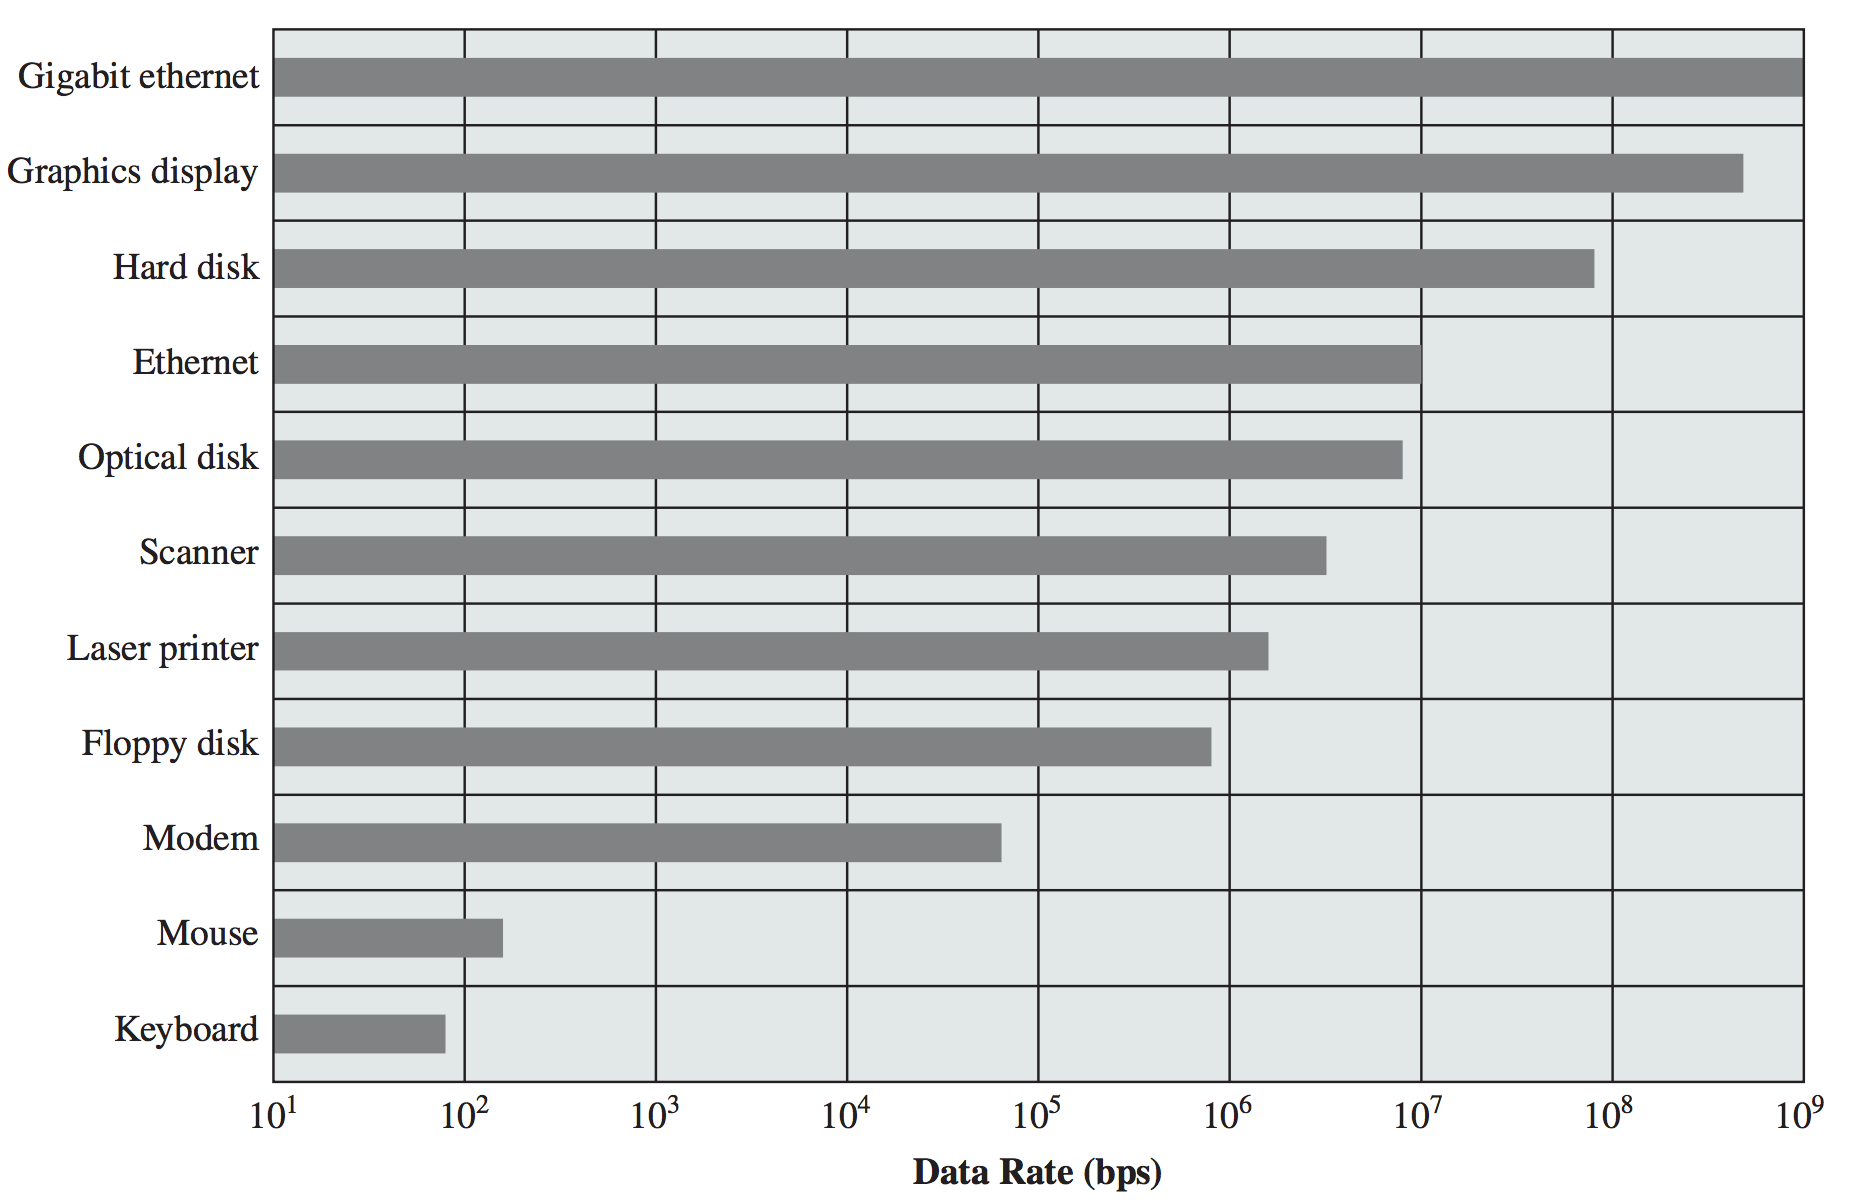
\includegraphics[width=\textwidth]{images/io-device-rates.png}
\end{center}


\end{frame}

\begin{frame}
\frametitle{I/O is Messy}

We might like to think that USB has taken away some of the complexity, but that's just the way a device connects to the computer. 

Managing the device itself is still as complicated as ever. 

All of the examples just listed can be connected via USB (Universal Serial Bus). 


\end{frame}

\begin{frame}
\frametitle{Disk vs General I/O}

Disk I/O has a huge impact on performance; it will receive its own discussion. 

But first, a little discussion about I/O in general.

\end{frame}

\begin{frame}
\frametitle{Disk vs General I/O}

For I/O the key parts are the bus and a controller. 

\begin{center}
	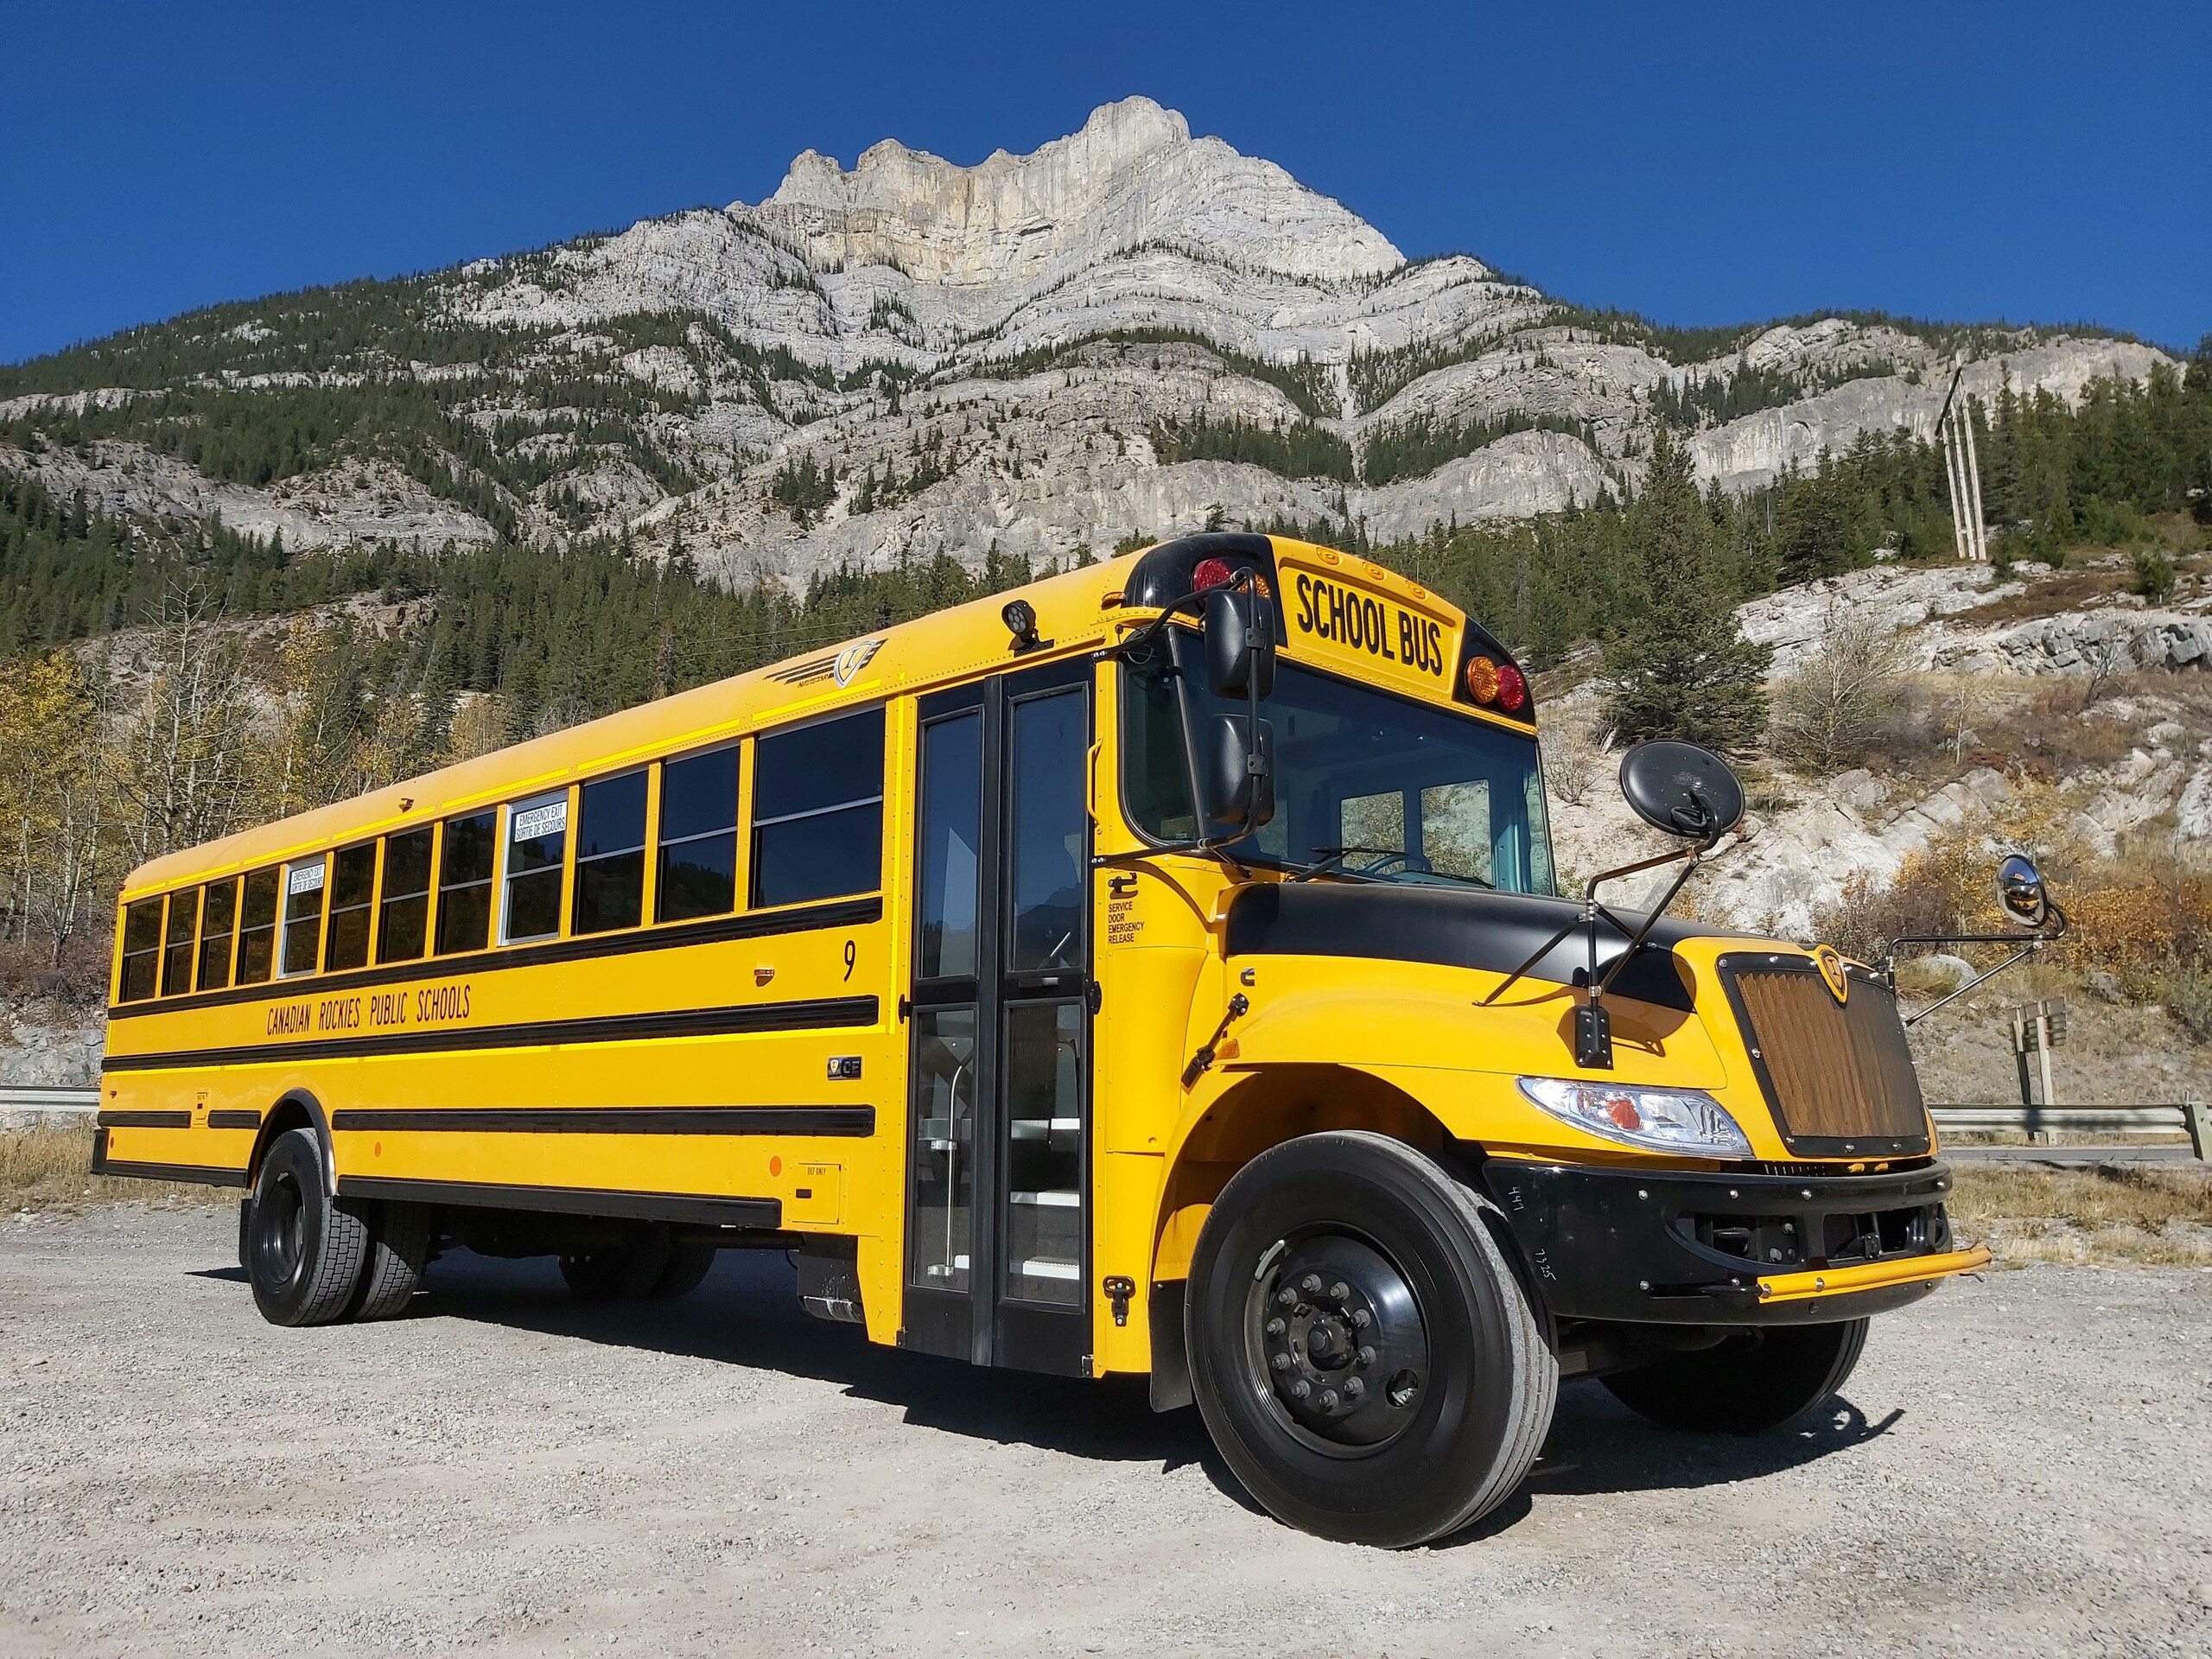
\includegraphics[width=0.3\textwidth]{images/bus.jpg}
	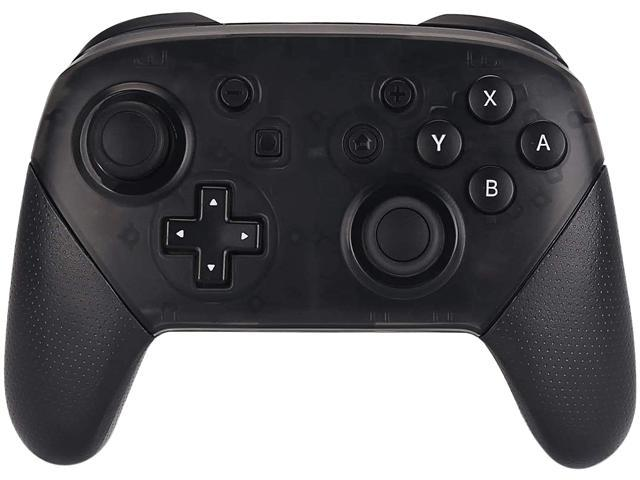
\includegraphics[width=0.3\textwidth]{images/controller.jpg}
\end{center}

After that there will be a protocol for how the devices will communicate\\
\quad e.g., polling, interrupts, or DMA.

\end{frame}


\begin{frame}
\frametitle{Quick Review}

Quick review of polling, interrupts, and DMA.\\
\quad Not all are equally good options in efficiency terms.

An I/O port represents the connection and may have 4 registers:\\
\quad data-in, data-out, status, control.

Main system is called \alert{host}.

\end{frame}


\begin{frame}
\frametitle{Polling}

Last choice, but might be our only choice!

Use a bit to mark the device as busy during operation.

Not exciting, but it does work.

\end{frame}


\begin{frame}
\frametitle{Polling}

Periodic polling might decrease CPU cycles but...

\begin{center}
	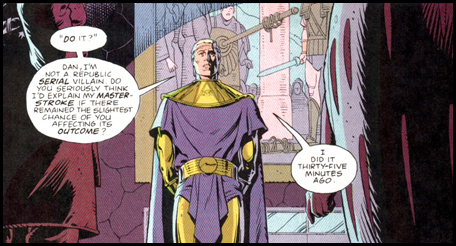
\includegraphics[width=0.75\textwidth]{images/watchmen.jpg}
\end{center}


\end{frame}


\begin{frame}
\frametitle{Interrupts}

There's some sort of interrupt request line (hardware) and when the CPU sees the signal that indicates the presence of an interrupt. 

Then the interrupt handler is executed to deal with it and clear the signal.

We'll dig into this topic soon!

\end{frame}


\begin{frame}
\frametitle{Something Something Fire Drill}

Ignores some complexity: interrupt priority, disabling interrupts?

But can avoid the problem of missing data.

\end{frame}


\begin{frame}
\frametitle{DMA}

Based on the idea of delegating the work to the DMA controller.

\begin{center}
	
\includegraphics[width=0.4\textwidth]{images/makeitso.jpg}
\end{center}

Can be quite efficient: CPU is still interrupted, but way less.

\end{frame}




\begin{frame}
\frametitle{Application I/O Interface}

Ideally a general-purpose operating system will accept new devices being added to the system without editing/reinstalling/recompiling the code. 

Your experience with object oriented programming gives you some familiarity with the solution of how we should accomplish this goal. 

We want to abstract away the details of the hardware, to the extent we can. 

Provide a uniform \alert{interface} to interact with. 

\end{frame}

\begin{frame}
\frametitle{I/O Interfaces}

In the very early days of operating systems, the hardware the computer shipped with was all the hardware it ever supported. 

If the vendor came out with a new module, they would have a new operating system update to introduce support for that device.


\end{frame}

\begin{frame}
\frametitle{I/O Interfaces} 

This got to be unmanageable in the era of the IBM PC because anybody could create hardware and attach it via a standard interface. 

Relying on IBM or Microsoft or whoever your OS vendor was to implement support for a random piece of hardware was not realistic.

\begin{center}
	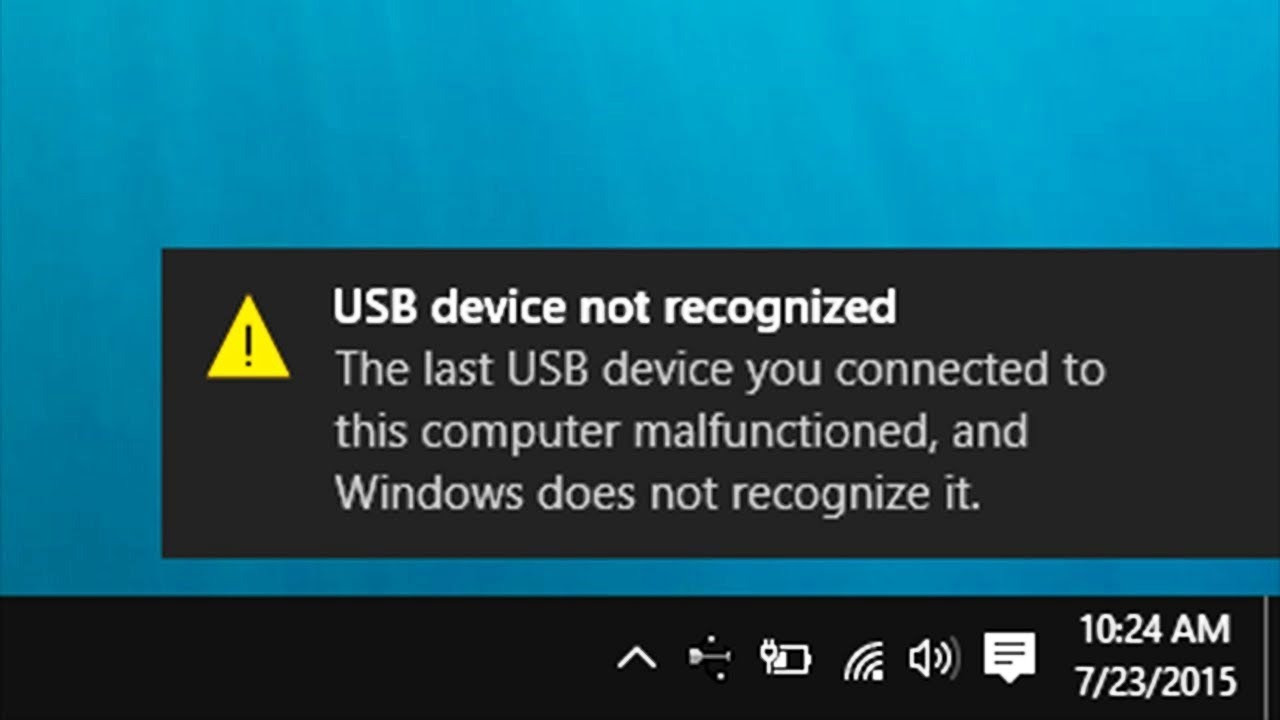
\includegraphics[width=0.5\textwidth]{images/notrecognized.jpg}
\end{center}

\end{frame}

\begin{frame}
\frametitle{I/O Interfaces}

Operating system developers thought they were very clever. 

They realized that they could shift the work to the hardware developers through a concept called \alert{device drivers}. 

\begin{center}
	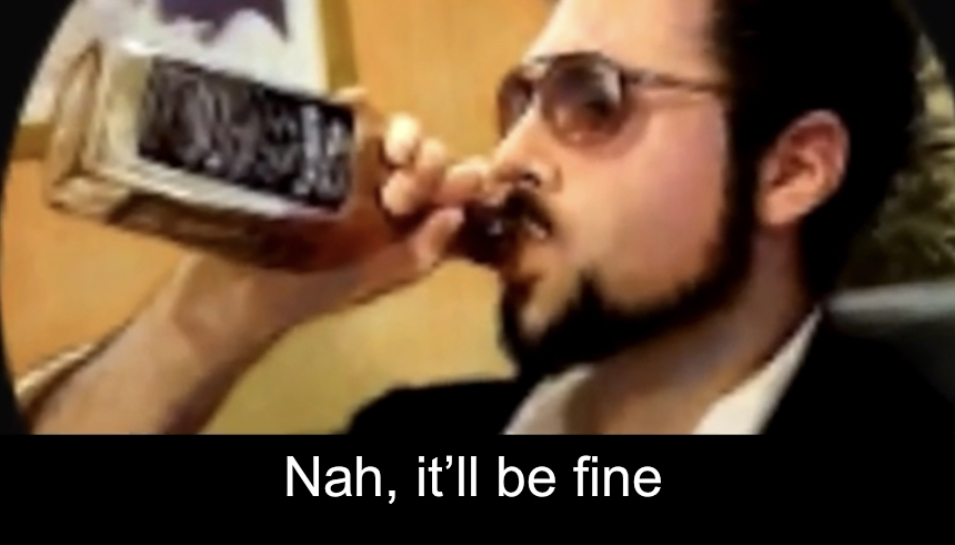
\includegraphics[width=0.4\textwidth]{images/befine.jpg}
\end{center}

\end{frame}

\begin{frame}
\frametitle{I/O Interfaces}

The device driver plugs in to the operating system through a standard interface. 

It tells the operating system a bit about the hardware and translates commands from the operating system to hardware instructions. 

Hardware developers often made extremely poor drivers.

\end{frame}

\begin{frame}
\frametitle{Device Drivers}

The problem was exacerbated by a Windows design decision.

Device drivers run in the system at the same protection level as the kernel. 

Some other operating systems have user-mode drivers, where possible or at an intermediate level between that of user space and the kernel. 

\end{frame}

\begin{frame}
\frametitle{Device Drivers}

\begin{center}
	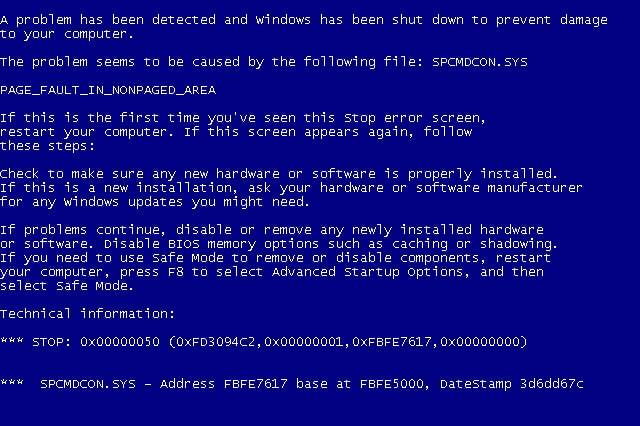
\includegraphics[width=0.7\textwidth]{images/bsod.jpg}
\end{center}

In Windows, a driver can invoke a system call that brings up everyone's favourite feature: the Blue Screen of Death (BSOD).

\end{frame}

\begin{frame}
\frametitle{Blue Screen of Death}

Microsoft, rightly or wrongly, was blamed for a lot of those BSODs. 

They took two approaches to remedy this problem. 

One was to write and include in Windows a lot more device drivers. 

\end{frame}

\begin{frame}
\frametitle{Blue Screen of Death}

The other was to introduce the static driver verifier; software used to test, at compile/build time, whether the driver will behave badly. 

Passing this test is required to get a sticker of approval from Microsoft.

\begin{center}
	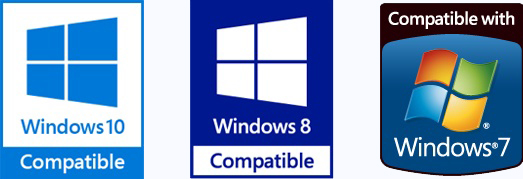
\includegraphics[width=0.5\textwidth]{images/wqhl.jpg}
\end{center}

The battle rages on about who is responsible for writing the drivers.


\end{frame}

\begin{frame}
\frametitle{Device Drivers}

Device drivers connect into the kernel's I/O subsystem to mediate between the kernel's I/O subsystem and the hardware device controller. 

\begin{center}
	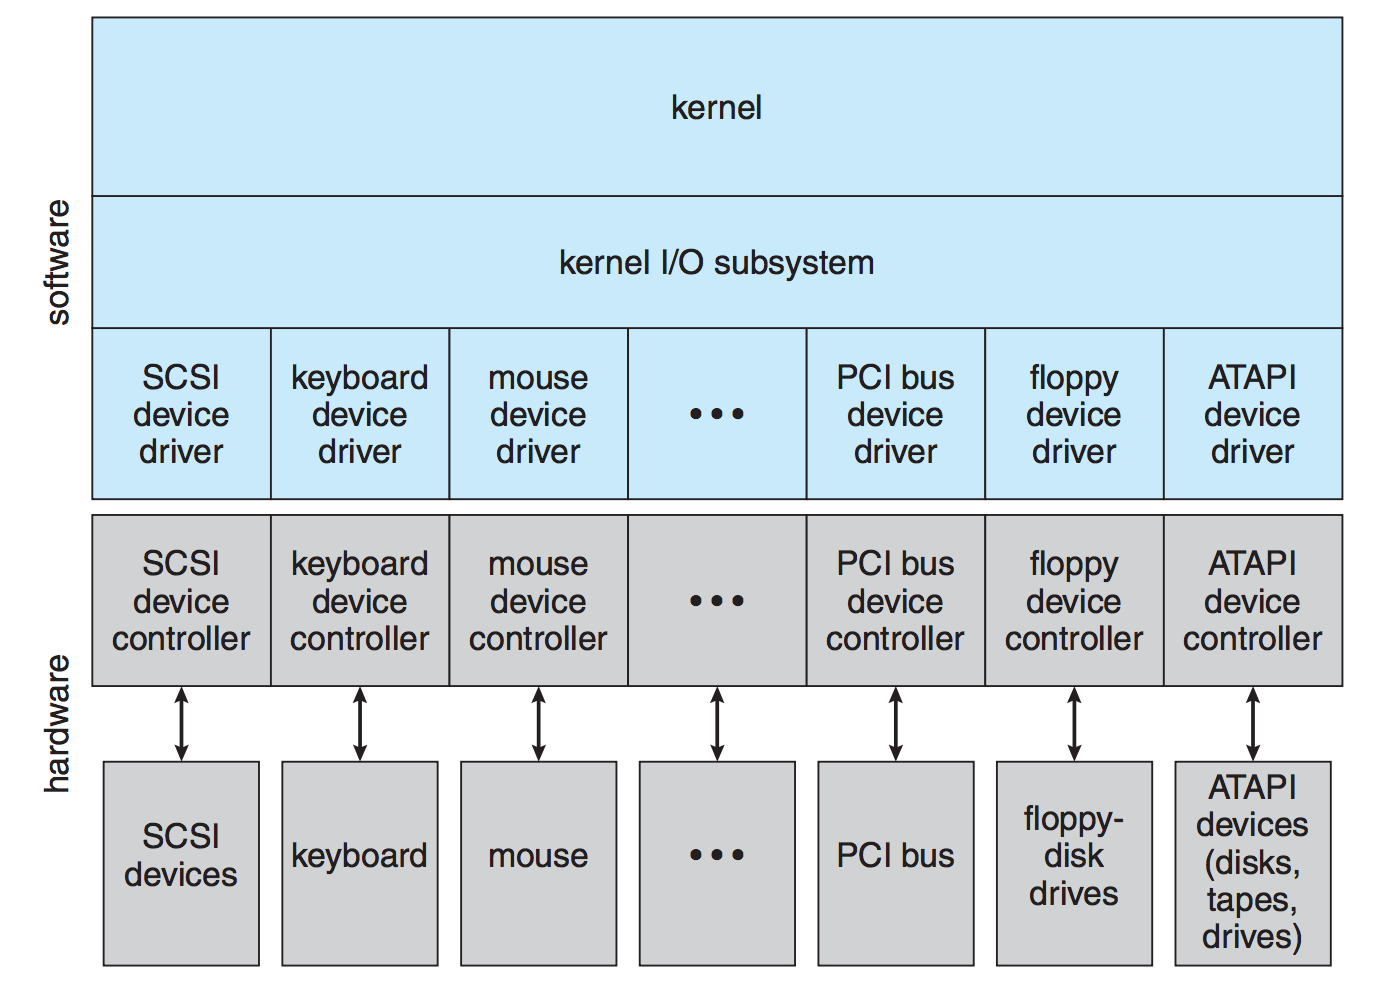
\includegraphics[width=0.75\textwidth]{images/kernel-io-structure.png}
\end{center}


\end{frame}

\begin{frame}
\frametitle{Abstraction}

Abstracting away details of the hardware makes the job of the OS dev easier.

Part of the difficulty is that devices can vary on numerous dimensions:

\begin{itemize}
\item \textbf{Data transfer mode}
\item \textbf{Access method}
\item \textbf{Transfer schedule}
\item \textbf{Dedication}
\item \textbf{Device Speed}
\item \textbf{Transfer Direction}
\end{itemize}

\end{frame}

\begin{frame}
\frametitle{Abstraction}

We would like to, as much as possible, keep the details above from the OS.

Devices will typically be grouped into a few categories so appropriate system calls can be issued. 

If a device is block-oriented, the OS should be issuing block read and write commands, not trying to do it one character at a time.


\end{frame}

\begin{frame}
\frametitle{Escape}

Operating systems also usually have an \alert{escape} system call that allows passing of a command directly from an application or the kernel to a device driver. 

This allows us to issue commands to a device that the OS designers have not thought of and created system calls for. 

\begin{center}
	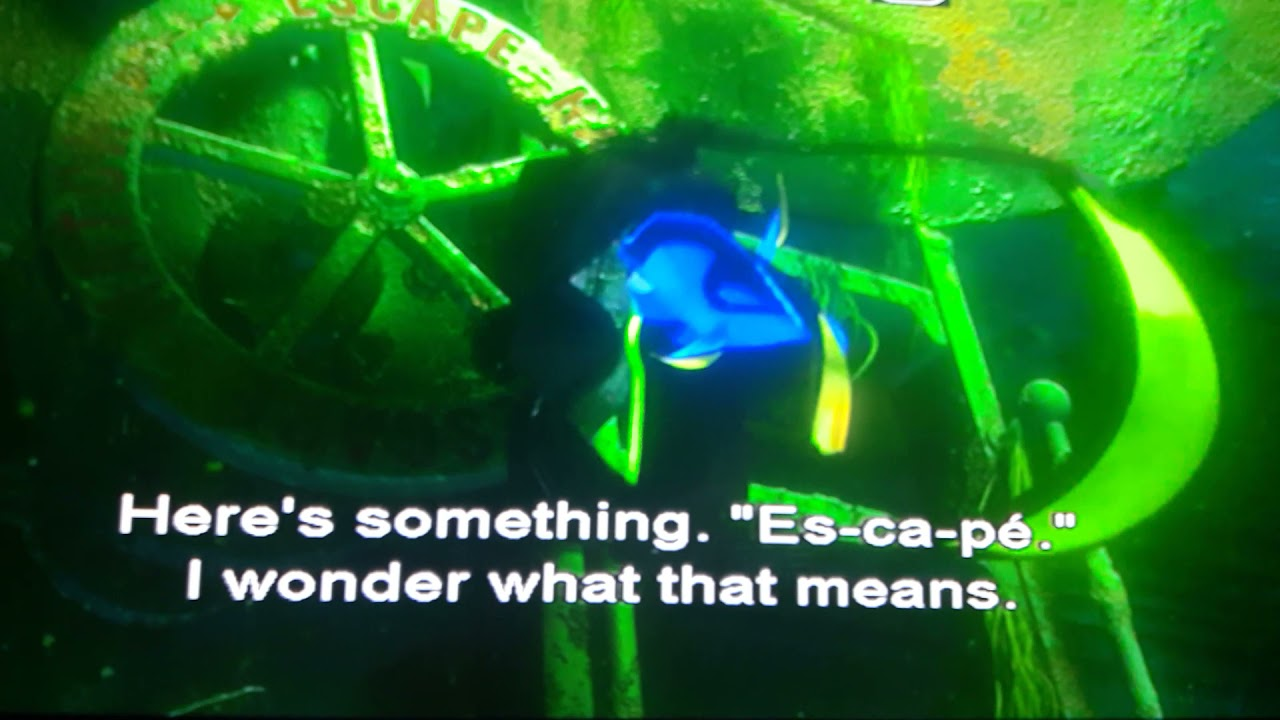
\includegraphics[width=0.5\textwidth]{images/escape-dory.jpg}
\end{center}

\end{frame}

\begin{frame}
\frametitle{Escape}


The UNIX system call for this is \texttt{ioctl} (``I/O Control''). 

It takes three parameters:\\
\quad A file descriptor indicating the hardware device.\\
\quad The command number\\
\quad A pointer to an arbitrary data structure that has control info \& data.

\end{frame}

\begin{frame}
\frametitle{Block and Character I/O}

The block device interface is used for block devices such as hard disk drives. 

Any device will support \texttt{read} and \texttt{write} commands, and if it is a random-access device, it will have a \texttt{seek} command to jump to a specific block. 

An application usually accesses the hard disk through the file system.

The OS can work on the hard drive using these 2/3 commands without being concerned with how that command is actually transmitted.

\end{frame}


\begin{frame}
\frametitle{Block and Character I/O}

We can abstract things a little bit further, from the perspective of the application developer, by having a memory-mapped file. 

Then, rather than using the block oriented operations directly, the application just writes to and reads from ``memory''.

The OS handles the behind-the-scene coordination to make writes go out to the correct block and read from the correct block.


\end{frame}

\begin{frame}
\frametitle{Block and Character I/O}

A character-oriented device is something like the keyboard.\\
\quad The system calls are \texttt{get} and \texttt{put}. 

Libraries and other structures may exist to work on a whole line at a time.

This is a good match for input devices that produce data in small amounts and at unpredictable times. 

Perhaps also for printers and sound output which operate naturally on a linear stream of bytes.

\end{frame}

\begin{frame}
\frametitle{Network Devices}

Network devices are fundamentally different from those that are directly attached to the system. 

Thus, the \texttt{read}, \texttt{write}, and \texttt{seek} routines are not really appropriate. 

The model in UNIX and Windows is that of \alert{sockets}.


\end{frame}


\begin{frame}
\frametitle{Socket To Me}

To support servers with multiple clients, the socket interface has a function \texttt{select}, that manages a set of sockets. 

Invoking this function returns information about what sockets have a packet waiting to be received and which are available for sending a packet. 

Proper use of \texttt{select} eliminates polling and busy-waiting in a situation where delays are unpredictable (which is always the case with the network).


\end{frame}

\begin{frame}
\frametitle{Spooling \& Reservations}

A \alert{spool} is a buffer for a device, like a printer, that can serve only 1 job at a time. 

Unlike disk, where it might read for $P_{1}$ now and then write for $P_{2}$ immediately afterwards, a printer needs to finish a whole print job before it starts the next. 

Printing is the most obvious example, but it is by no means the only one. 

The operating system centralizes all communication to the printer and runs it through the spooling system. 


\end{frame}



\begin{frame}
\frametitle{I/O Protection}

Recall from much earlier the idea of kernel mode and user mode instructions. 

We want all user accesses to I/O to be mediated through the operating system, so the OS can check to see if the request is valid. 

This helps minimize errors and problems where people do bad things like cancel another process's request so theirs can go first. 

Our typical tradeoff: increased safety in exchange for reduced performance.

\end{frame}

\end{document}

